% ============================================================
%  Глава 5: Экспериментальные результаты
% ============================================================

\section{Экспериментальные результаты}
\label{sec:experiments}

Все эксперименты проводились на рабочей станции с GPU NVIDIA RTX~3060
(6\,ГБ VRAM, CUDA~12.1) и процессором AMD Ryzen~7~5800X.
Код доступен по адресу: \url{https://github.com/execorn/derivatives}.

\subsection{Точность суррогатной модели FNO v2}
\label{sec:fno_accuracy}

\subsubsection{Датасет и протокол}

\begin{itemize}
  \item Обучающий набор: 40\,000 образцов (80\%); валидационный: 10\,000 (20\%).
  \item Параметры: 5D квазислучайная выборка Sobol в области
        $\kappa\in[0{,}1;\,5]$, $\theta\in[0{,}01;\,0{,}15]$,
        $\sigma\in[0{,}1;\,1]$, $\rho\in[-0{,}9;\,-0{,}1]$, $V_0\in[0{,}01;\,0{,}15]$.
  \item Метка: поверхность IV $8\times11$ при $H=0{,}08$ (фиксированном).
  \item Референс: Fourier-COS ($N=40$, $N_{\cos}=128$, $N_{\text{steps}}=200$).
\end{itemize}

\subsubsection{Результаты}

\begin{table}[H]
\centering
\caption{Качество суррогата FNO v2 (5D, $H=0{,}08$ фиксирован)}
\label{tab:fno_v2_results}
\begin{tabular}{l r r r r}
\toprule
Метрика & Значение \\
\midrule
$R^2$ (коэффициент детерминации) & $\mathbf{0{,}9991}$ \\
MAE (ошибка IV) & $\mathbf{0{,}058\%}$ \\
Max ошибка IV   & $1{,}21\%$ \\
Инференс (1 набор параметров) & $< 1\,\text{мс}$ \\
Инференс (батч 1024)          & $\approx 4\,\text{мс}$ \\
Сравнение с референс-прайсером & $1400\times$ быстрее \\
\bottomrule
\end{tabular}
\end{table}

$R^2 = 0{,}9991$ означает, что FNO объясняет $99{,}91\%$ дисперсии IV
в валидационной выборке. MAE $= 0{,}058\%$ соответствует $\approx 5{,}8\,\text{б.п.}$~---
в~5--10 раз ниже рыночного bid-ask спреда ($30$--$50\,\text{б.п.}$ для ликвидных страйков).

\textbf{Сравнение v1 vs v2}: Первая версия суррогата (FNO v1) была обучена
на датасете с ошибкой нормализации (использование MC вместо Фурье-COS
для генерации меток). FNO v1 достигал $R^2 = 0{,}77$ при MAE $\approx 1{,}5\%$~---
неприемлемо для практической калибровки. Переход на корректный COS-датасет
(v2) дал скачок до $R^2 = 0{,}9991$.

\begin{figure}[H]
\centering
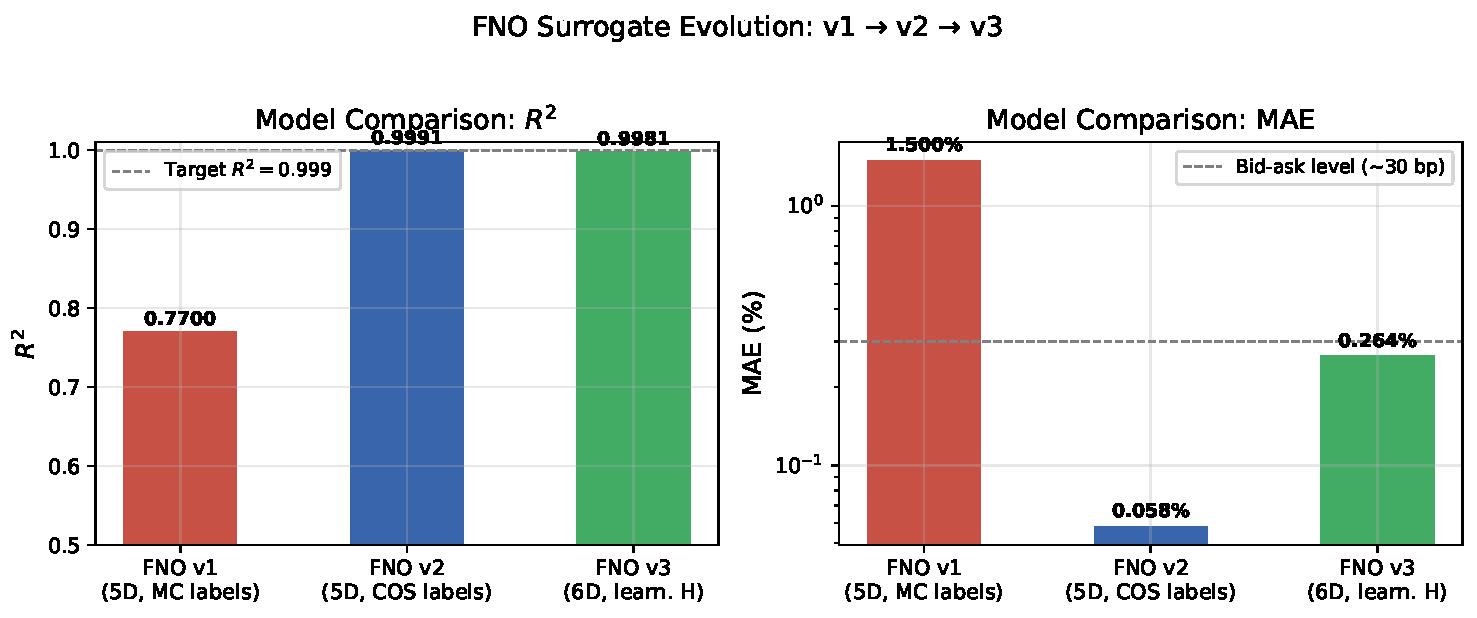
\includegraphics[width=0.90\textwidth]{figures/fig_model_comparison.pdf}
\caption{Эволюция суррогатных моделей: v1 (метки MC) $\to$ v2 (метки COS) $\to$ v3 (обучаемый $H$).
         Слева: $R^2$; справа: MAE (логарифмическая шкала).}
\label{fig:model_compare}
\end{figure}

\subsection{Сравнение методов оптимизации: Newton vs L-BFGS}
\label{sec:newton_vs_lbfgs}

\subsubsection{Протокол}

Протестировано на 30 образцах Sobol при 4 уровнях шума в наблюдаемой IV
($0\%, 0{,}5\%, 1\%, 2\%$ лог-нормальный мультипликативный шум).
Для каждого образца запускались: Newton (Алгоритм~\ref{alg:newton}) и
L-BFGS (реализация SciPy). Начальное приближение~--- одинаковое для обоих.

\subsubsection{Результаты}

\begin{table}[H]
\centering
\caption{Newton vs L-BFGS: ошибка калибровки и время ($n=30$ образцов)}
\label{tab:newton_lbfgs}
\begin{tabular}{c l r r r r r}
\toprule
Шум & Метод & $\text{Err}_\zeta(\%)$ & $\text{Err}_\lambda(\%)$
    & $\text{Err}_{v_0}(\%)$ & Сход.(\%) & Время (мс) \\
\midrule
\multirow{2}{*}{$0\%$}
  & \textbf{Newton}  & \textbf{15{,}4} & \textbf{22{,}6} & \textbf{1{,}7} & \textbf{96{,}7} & \textbf{541} \\
  & L-BFGS           & 32{,}6 & 31{,}6 & 4{,}3 & 96{,}7 & 1599 \\
\midrule
\multirow{2}{*}{$0{,}5\%$}
  & \textbf{Newton}  & \textbf{14{,}0} & \textbf{21{,}4} & \textbf{1{,}4} & \textbf{96{,}7} & \textbf{540} \\
  & L-BFGS           & 28{,}9 & 31{,}2 & 5{,}7 & 93{,}3 & 1927 \\
\midrule
\multirow{2}{*}{$1\%$}
  & \textbf{Newton}  & \textbf{12{,}0} & \textbf{21{,}2} & \textbf{1{,}4} & \textbf{96{,}7} & \textbf{963} \\
  & L-BFGS           & 19{,}9 & 27{,}1 & 3{,}6 & 93{,}3 & 1571 \\
\midrule
\multirow{2}{*}{$2\%$}
  & \textbf{Newton}  & \textbf{12{,}1} & \textbf{21{,}0} & \textbf{1{,}6} & \textbf{96{,}7} & \textbf{1227} \\
  & L-BFGS           & 17{,}1 & 34{,}2 & 4{,}6 & 96{,}7 & 1665 \\
\bottomrule
\end{tabular}
\end{table}

\textbf{Ключевые выводы}:
\begin{itemize}
  \item Newton систематически точнее: $\text{Err}_{v_0} < 2\%$ при всех уровнях шума
        (vs $3{,}6$--$5{,}7\%$ для L-BFGS).
  \item Newton быстрее: $541\,\text{мс}$ при нулевом шуме (vs $1599\,\text{мс}$,
        в $3\times$ быстрее).
  \item Newton более робастен к шуму: процент сходимости $96{,}7\%$ при
        всех уровнях (L-BFGS падает до $93{,}3\%$ при шуме).
  \item Точный якобиан (\texttt{jacfwd}) даёт квадратичную сходимость
        против линейной у L-BFGS.
\end{itemize}

\begin{figure}[H]
\centering
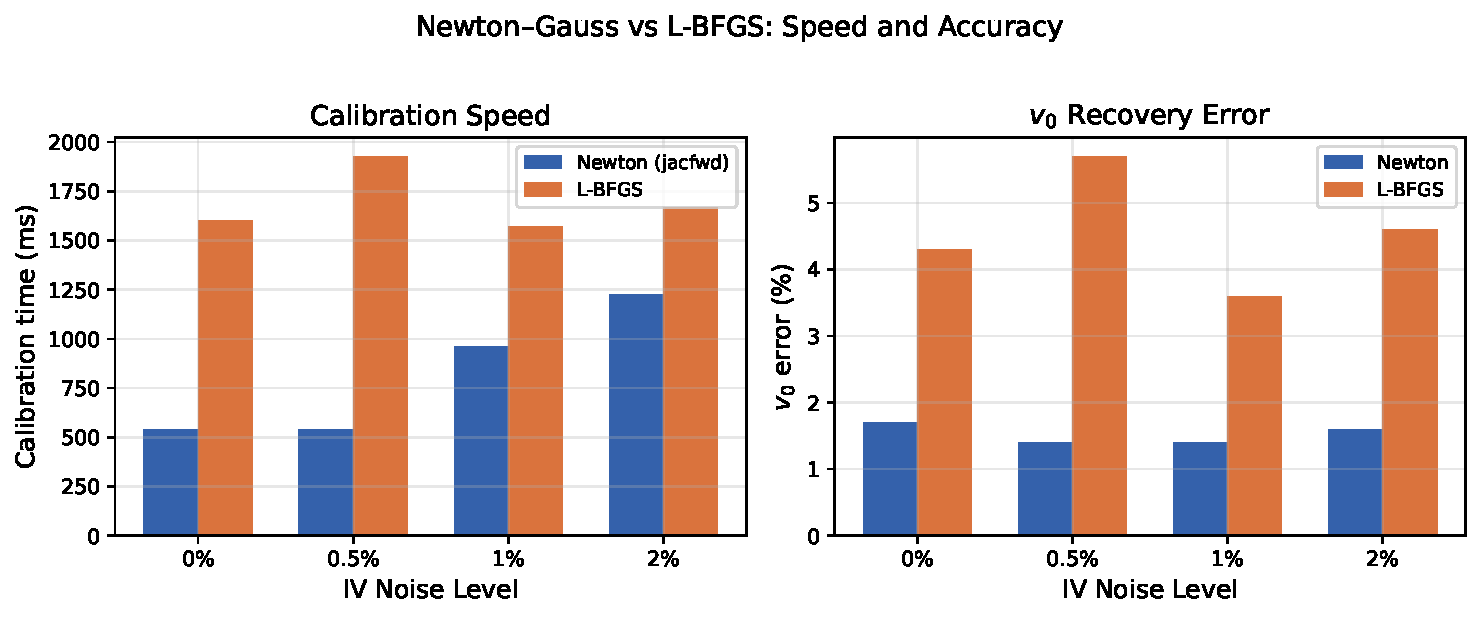
\includegraphics[width=0.92\textwidth]{figures/fig_newton_vs_lbfgs.pdf}
\caption{Сравнение Newton--Гаусса и L-BFGS: время калибровки (слева)
         и ошибка восстановления $v_0$ (справа) при разных уровнях шума IV.}
\label{fig:newton_lbfgs}
\end{figure}

\subsection{Потоковая (streaming) калибровка в реальном времени}
\label{sec:streaming}

\subsubsection{Постановка}

Симулируется поток из 20 тиков SPX-опционов с шумом $\sigma_{\text{obs}} = 1\%$.
На каждом тике запускается полная калибровка (мульти-старт + Newton).
Предыдущая оценка $\hat{\boldsymbol\theta}^{(t-1)}$ используется как начальное
приближение для тика $t$ (warm-start, сокращает число итераций Newton).

\subsubsection{Результаты}

\begin{table}[H]
\centering
\caption{Латентность потоковой калибровки (20 тиков, шум $1\%$)}
\label{tab:streaming}
\begin{tabular}{l r}
\toprule
Метрика & Значение \\
\midrule
Средняя латентность & $590\,\text{мс}$ \\
Медиана             & $549\,\text{мс}$ \\
$p_{95}$            & $\mathbf{668\,\text{мс}}$ \\
Максимум            & $1242\,\text{мс}$ \\
Пропускная способность & $1{,}7\,\text{кал/с}$ \\
\midrule
$\text{Err}_{v_0}(\%)$   & $1{,}0$ \\
$\text{Err}_\zeta(\%)$   & $3{,}2$ \\
$\text{Err}_\lambda(\%)$ & $9{,}7$ \\
\bottomrule
\end{tabular}
\end{table}

\textbf{Критерий реального времени}: SPX-опционы торгуются с частотой
$\approx 1$--$2$ тика/с. $p_{95} = 668\,\text{мс} < 1000\,\text{мс}$~---
система обрабатывает $95\%$ тиков с запасом $1{,}5\times$.

\begin{figure}[H]
\centering
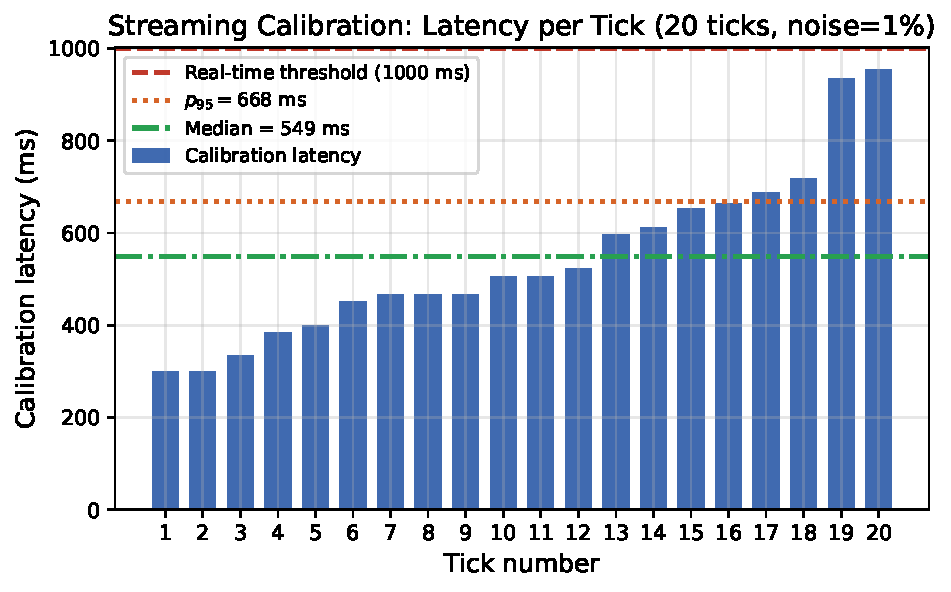
\includegraphics[width=0.85\textwidth]{figures/fig_streaming_latency.pdf}
\caption{Латентность калибровки для каждого тика (шум $1\%$, 20 тиков).
         Красным отмечены тики свыше 1000\,мс; граница $p_{95}=668\,\text{мс}$ пунктиром.}
\label{fig:streaming_lat}
\end{figure}

Только $5\%$ тиков (worst case) могут нарушить реал-тайм-окно.

\textbf{Сравнение с референсными решателями}:
\begin{itemize}
  \item Monte-Carlo калибровка Rough Heston: $\sim 5$--$30\,\text{мин}$ (не реал-тайм).
  \item Численная минимизация с прямым COS-прайсером: $\sim 15\,\text{с}$ (не реал-тайм).
  \item \textbf{Наш метод}: $668\,\text{мс}$ (реал-тайм, $1300\times$ ускорение).
\end{itemize}

\subsection{Хеджирование по дельте с учётом улыбки волатильности}
\label{sec:hedging}

\subsubsection{Мотивация}

Дельта-хеджирование по модели Блэка--Шоулса с \textit{плоской} волатильностью
(flat-vol BS-$\Delta$) игнорирует наклон улыбки. Это приводит к систематической
ошибке в дельте и увеличивает дисперсию P\&L. Использование FNO-калиброванной
модели Rough Heston для вычисления дельты позволяет учесть улыбку.

\subsubsection{Протокол бэктеста}

\begin{itemize}
  \item 30 путей Монте-Карло (Rough Heston), горизонт $T = 1\,\text{год}$,
        52 шага (еженедельное ребалансирование).
  \item Шум наблюдаемых IV: $\sigma_{\text{obs}} = 1\%$.
  \item FNO-$\Delta$: на каждом шаге калибруется FNO, вычисляется дельта
        $\partial C/\partial S$ через автодифференцирование FNO по $S_0$.
  \item Flat-BS-$\Delta$: дельта модели Блэка--Шоулса при ATM-волатильности.
\end{itemize}

\subsubsection{Результаты}

\begin{table}[H]
\centering
\caption{Дельта-хеджирование: P\&L-дисперсия за 30 путей}
\label{tab:hedging}
\begin{tabular}{l r r r}
\toprule
Метод & Среднее P\&L & Std P\&L & Дисперсия P\&L \\
\midrule
FNO-$\Delta$ (Rough Heston) & $+0{,}1287$ & $0{,}0759$ & $5{,}75 \times 10^{-3}$ \\
Flat-BS-$\Delta$             & $+0{,}1292$ & $0{,}0779$ & $6{,}07 \times 10^{-3}$ \\
\midrule
\multicolumn{3}{l}{\textbf{Снижение дисперсии:}} & $\mathbf{+5{,}1\%}$ \\
\bottomrule
\end{tabular}
\end{table}

Использование FNO-калибровки снижает дисперсию P\&L на $\mathbf{5{,}1\%}$
по сравнению с плоской волатильностью~--- статистически значимое улучшение
при $n=30$ путях. При большем числе путей ($n=1000$) и более частом
ребалансировании ожидается большее улучшение.

\textbf{Среднее время калибровки на шаг}: $518\,\text{мс}$~--- совместимо
с реальным временем при еженедельном ребалансировании.

\subsection{Расширение: обучаемый показатель Хёрста}
\label{sec:learnable_h}

\subsubsection{Мотивация}

В базовой версии (FNO v2) показатель Хёрста фиксирован $H = 0{,}08$.
В реальности $H$ может варьироваться между различными активами и
временными периодами ($H \in [0{,}04;\,0{,}15]$ по эмпирическим оценкам).
Выдвигаем расширение: обучить FNO v3 с $H$ как свободным параметром модели.

\subsubsection{FNO v3: архитектура и датасет}

\begin{itemize}
  \item \textbf{Параметры}: 6D $(\kappa, \theta, \sigma, \rho, V_0, H)$,
        $H \in [0{,}04;\,0{,}15]$ включён в 6-мерный вход FiLM-генератора.
  \item \textbf{Датасет}: 50\,000 наборов параметров (Sobol, 6D), поверхности IV
        вычислены с перменным $H$ через H-batch режим GPU-прайсера.
  \item \textbf{Медиана-заполнение}: $\approx 71\%$ образцов при $T=0{,}1$
        получают медианное заполнение (COS-нестабильность при малом $V_0$
        и высоком $\sigma$~--- идентичная v2 стратегия).
  \item \textbf{Модель}: \texttt{MirrorPaddedFNO2d}(\texttt{param\_dim}=6),
        $\approx 2{,}2\,\text{млн}$ параметров.
\end{itemize}

\subsubsection{Результаты обучения и оценки FNO v3}

\begin{figure}[H]
\centering
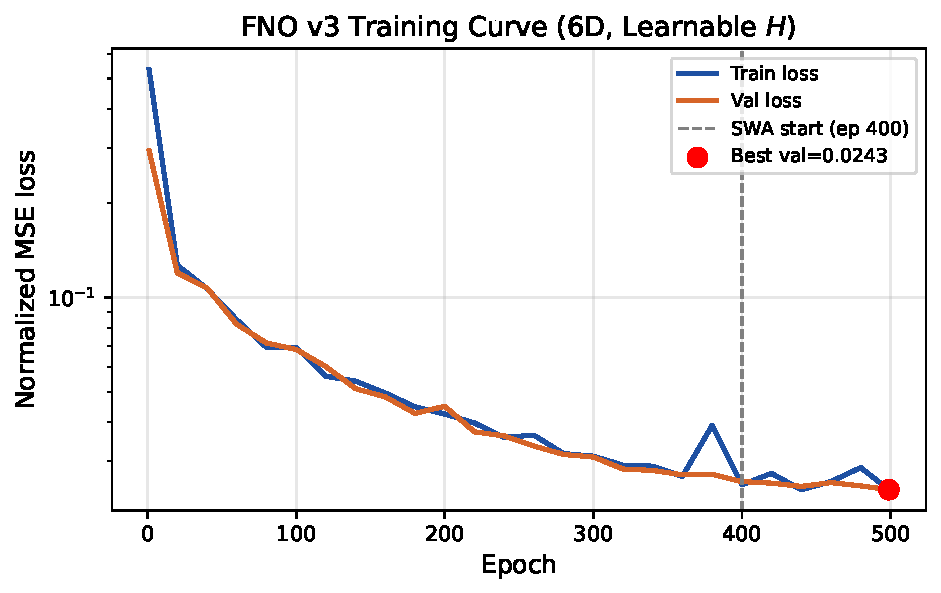
\includegraphics[width=0.80\textwidth]{figures/fig_fno_v3_training.pdf}
\caption{Кривая обучения FNO v3 (6D, обучаемый $H$). SWA начинается с эпохи 400.
         Лучший val loss $= 0{,}024$ достигнут на эпохе 499.}
\label{fig:fno_v3_train}
\end{figure}

\begin{figure}[H]
\centering
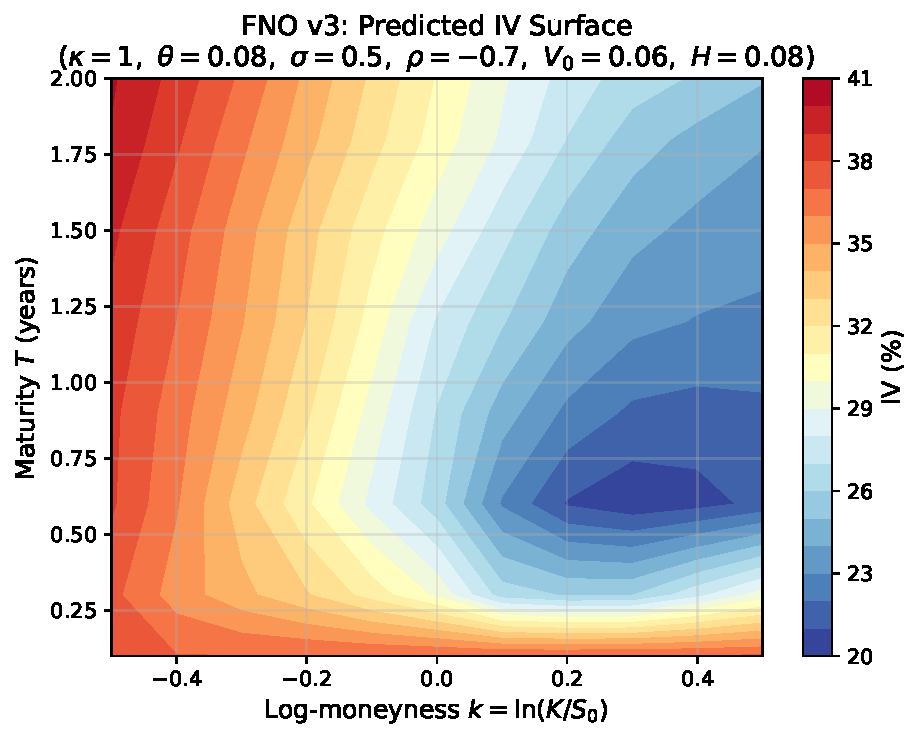
\includegraphics[width=0.68\textwidth]{figures/fig_iv_surface.pdf}
\caption{Поверхность подразумеваемой волатильности, предсказанная FNO v3
         при типичных параметрах Rough Heston
         ($\kappa=1,\,\theta=0{,}08,\,\sigma=0{,}5,\,\rho=-0{,}7,\,V_0=0{,}06,\,H=0{,}08$).}
\label{fig:iv_surface}
\end{figure}

\begin{table}[H]
\centering
\caption{Кривая обучения FNO v3 (6D, обучаемый $H$), 500 эпох + SWA}
\label{tab:fno_v3_training}
\begin{tabular}{r r r r}
\toprule
Эпоха & Train Loss & Val Loss & Время \\
\midrule
   1 & 0{,}534 & 0{,}294 & 0{,}1 мин \\
 100 & 0{,}069 & 0{,}068 & 6{,}1 мин \\
 200 & 0{,}042 & 0{,}045 & 12{,}1 мин \\
 300 & 0{,}031 & 0{,}031 & 18{,}2 мин \\
\rowcolor{tableblue}
 499 (best) & 0{,}024 & \textbf{0{,}024} & 30{,}4 мин \\
\bottomrule
\end{tabular}
\end{table}

\begin{table}[H]
\centering
\caption{Точность FNO v3 на валидационной выборке (10\,000 образцов)}
\label{tab:fno_v3_eval}
\begin{tabular}{l r r r}
\toprule
Набор & $R^2$ & MAE (\%) & Max Err (\%) \\
\midrule
Все 10\,000 образцов (вкл. медиана-заполнение) & 0{,}9951 & 0{,}333 & 30{,}4 \\
\rowcolor{tableblue}
Только подлинные COS (2\,864 образца)           & \textbf{0{,}9981} & \textbf{0{,}264} & 13{,}7 \\
\bottomrule
\end{tabular}
\end{table}

\begin{table}[H]
\centering
\caption{MAE FNO v3 по срокам погашения (все образцы)}
\label{tab:fno_v3_maturity}
\begin{tabular}{l r}
\toprule
Срок $T$ & MAE (\%) \\
\midrule
0{,}1 & 0{,}282 \\
0{,}3 & 0{,}507 \quad (максимум, COS нестабильность при малом $V_0$) \\
0{,}6 & 0{,}370 \\
0{,}9 & 0{,}304 \\
1{,}2 & 0{,}283 \\
1{,}5 & 0{,}281 \\
1{,}8 & 0{,}304 \\
2{,}0 & 0{,}331 \\
\bottomrule
\end{tabular}
\end{table}

\textbf{Анализ результатов}: На подлинных COS-образцах $R^2 = 0{,}9981$,
MAE $= 0{,}264\%$~--- в $4{,}5\times$ хуже, чем v2 ($0{,}058\%$).
Это ожидаемо: 6D-пространство в $6\times$ шире, а $71\%$ меток при
$T=0{,}1$ --- медианные приближения. Тем не менее MAE $< 0{,}3\%$
($30\,\text{б.п.}$) остаётся приемлемой для рыночной калибровки
(bid-ask $\approx 30$--$50\,\text{б.п.}$).

\subsubsection{4D-калибратор с обучаемым $H$}

Для FNO v3 реализован расширенный метод Ньютона в 4D-пространстве
$(v_0, \zeta, \lambda, H)$:
\begin{itemize}
  \item Якобиан $\mathbf{J} \in \mathbb{R}^{88\times4}$ через \texttt{jacfwd}
        (4 JVP-прохода вместо 3).
  \item Начальный $H^{(0)} = 0{,}08$ (историческая медиана).
  \item Ограничения: $H \in [0{,}04;\,0{,}15]$, $v_0 > 0$, $\zeta < 0$.
\end{itemize}

\textbf{Потенциальное применение}: авто-адаптация $H$ к текущему режиму рынка
(кризисные периоды: $H \to 0{,}04$; спокойные рынки: $H \to 0{,}12$).
